% *** Authors should verify (and, if needed, correct) their LaTeX system  ***
% *** with the testflow diagnostic prior to trusting their LaTeX platform ***
% *** with production work. IEEE's font choices can trigger bugs that do  ***
% *** not appear when using other class files.                            ***
% The testflow support page is at:
% http://www.michaelshell.org/tex/testflow/


%%*************************************************************************
%% Legal Notice:
%% This code is offered as-is without any warranty either expressed or
%% implied; without even the implied warranty of MERCHANTABILITY or
%% FITNESS FOR A PARTICULAR PURPOSE!
%% User assumes all risk.
%% In no event shall IEEE or any contributor to this code be liable for
%% any damages or losses, including, but not limited to, incidental,
%% consequential, or any other damages, resulting from the use or misuse
%% of any information contained here.
%%
%% All comments are the opinions of their respective authors and are not
%% necessarily endorsed by the IEEE.
%%
%% This work is distributed under the LaTeX Project Public License (LPPL)
%% ( http://www.latex-project.org/ ) version 1.3, and may be freely used,
%% distributed and modified. A copy of the LPPL, version 1.3, is included
%% in the base LaTeX documentation of all distributions of LaTeX released
%% 2003/12/01 or later.
%% Retain all contribution notices and credits.
%% ** Modified files should be clearly indicated as such, including  **
%% ** renaming them and changing author support contact information. **
%%
%% File list of work: IEEEtran.cls, New_IEEEtran_how-to.pdf, bare_jrnl_new_sample4.tex,
%%*************************************************************************
\PassOptionsToPackage{unicode}{hyperref}
\PassOptionsToPackage{hyphens}{url}
\PassOptionsToPackage{dvipsnames,svgnames,x11names}{xcolor}
% Note that the a4paper option is mainly intended so that authors in
% countries using A4 can easily print to A4 and see how their papers will
% look in print - the typesetting of the document will not typically be
% affected with changes in paper size (but the bottom and side margins will).
% Use the testflow package mentioned above to verify correct handling of
% both paper sizes by the user's LaTeX system.
%
% Also note that the "draftcls" or "draftclsnofoot", not "draft", option
% should be used if it is desired that the figures are to be displayed in
% draft mode.
%
\documentclass[
  journal,
]{IEEEtran}%
% If IEEEtran.cls has not been installed into the LaTeX system files,
% manually specify the path to it like:
% \documentclass[journal]{../sty/IEEEtran}
\usepackage[cmex10]{amsmath}
\usepackage{amssymb}
\usepackage{iftex}
\ifPDFTeX
  \usepackage[T1]{fontenc}
  \usepackage[utf8]{inputenc}
  \usepackage{textcomp} % provide euro and other symbols
\else % if luatex or xetex
  \usepackage{unicode-math} % this also loads fontspec
  \defaultfontfeatures{Scale=MatchLowercase}
  \defaultfontfeatures[\rmfamily]{Ligatures=TeX,Scale=1}
\fi
%\usepackage{lmodern}
\ifPDFTeX\else
\fi
% Use upquote if available, for straight quotes in verbatim environments
\IfFileExists{upquote.sty}{\usepackage{upquote}}{}
\IfFileExists{microtype.sty}{% use microtype if available
  \usepackage[]{microtype}
  \UseMicrotypeSet[protrusion]{basicmath} % disable protrusion for tt fonts
}{}
\makeatletter
\parindent    1.0em
\ifCLASSOPTIONcompsoc
  \parindent    1.5em
\fi
\makeatother
\usepackage{xcolor}
\setlength{\emergencystretch}{3em} % prevent overfull lines

\setcounter{secnumdepth}{5}
% Make \paragraph and \subparagraph free-standing
\ifx\paragraph\undefined\else
  \let\oldparagraph\paragraph
  \renewcommand{\paragraph}[1]{\oldparagraph{#1}\mbox{}}
\fi
\ifx\subparagraph\undefined\else
  \let\oldsubparagraph\subparagraph
  \renewcommand{\subparagraph}[1]{\oldsubparagraph{#1}\mbox{}}
\fi

\usepackage{longtable,booktabs,array}
\newcounter{none} % for unnumbered tables
\usepackage{calc} % for calculating minipage widths
% Correct order of tables after \paragraph or \subparagraph
\usepackage{etoolbox}
\makeatletter
\patchcmd\longtable{\par}{\if@noskipsec\mbox{}\fi\par}{}{}
\makeatother
% Allow footnotes in longtable head/foot
\IfFileExists{footnotehyper.sty}{\usepackage{footnotehyper}}{\usepackage{footnote}}
\makesavenoteenv{longtable}
\usepackage{graphicx}
\makeatletter
\newsavebox\pandoc@box
\newcommand*\pandocbounded[1]{% scales image to fit in text height/width
  \sbox\pandoc@box{#1}%
  \Gscale@div\@tempa{\textheight}{\dimexpr\ht\pandoc@box+\dp\pandoc@box\relax}%
  \Gscale@div\@tempb{\linewidth}{\wd\pandoc@box}%
  \ifdim\@tempb\p@<\@tempa\p@\let\@tempa\@tempb\fi% select the smaller of both
  \ifdim\@tempa\p@<\p@\scalebox{\@tempa}{\usebox\pandoc@box}%
  \else\usebox{\pandoc@box}%
  \fi%
}
% Set default figure placement to htbp
\def\fps@figure{htbp}
\makeatother


% definitions for citeproc citations
\NewDocumentCommand\citeproctext{}{}
\NewDocumentCommand\citeproc{mm}{%
  \begingroup\def\citeproctext{#2}\cite{#1}\endgroup}
\makeatletter
 % allow citations to break across lines
 \let\@cite@ofmt\@firstofone
 % avoid brackets around text for \cite:
 \def\@biblabel#1{}
 \def\@cite#1#2{{#1\if@tempswa , #2\fi}}
\makeatother
\newlength{\cslhangindent}
\setlength{\cslhangindent}{1.5em}
\newlength{\csllabelwidth}
\setlength{\csllabelwidth}{3em}
\newenvironment{CSLReferences}[2] % #1 hanging-indent, #2 entry-spacing
 {\begin{list}{}{%
  \setlength{\itemindent}{0pt}
  \setlength{\leftmargin}{0pt}
  \setlength{\parsep}{0pt}
  % turn on hanging indent if param 1 is 1
  \ifodd #1
   \setlength{\leftmargin}{\cslhangindent}
   \setlength{\itemindent}{-1\cslhangindent}
  \fi
  % set entry spacing
  \setlength{\itemsep}{#2\baselineskip}}}
 {\end{list}}
\usepackage{calc}
\newcommand{\CSLBlock}[1]{\hfill\break\parbox[t]{\linewidth}{\strut\ignorespaces#1\strut}}
\newcommand{\CSLLeftMargin}[1]{\parbox[t]{\csllabelwidth}{\strut#1\strut}}
\newcommand{\CSLRightInline}[1]{\parbox[t]{\linewidth - \csllabelwidth}{\strut#1\strut}}
\newcommand{\CSLIndent}[1]{\hspace{\cslhangindent}#1}



\setlength{\emergencystretch}{3em} % prevent overfull lines

\providecommand{\tightlist}{%
  \setlength{\itemsep}{0pt}\setlength{\parskip}{0pt}}



 


\usepackage{physics}
\usepackage[version=3]{mhchem}
\usepackage{orcidlink}
\usepackage{float}
\floatplacement{table}{htb}
\makeatletter
\@ifpackageloaded{caption}{}{\usepackage{caption}}
\AtBeginDocument{%
\ifdefined\contentsname
  \renewcommand*\contentsname{Table of contents}
\else
  \newcommand\contentsname{Table of contents}
\fi
\ifdefined\listfigurename
  \renewcommand*\listfigurename{List of Figures}
\else
  \newcommand\listfigurename{List of Figures}
\fi
\ifdefined\listtablename
  \renewcommand*\listtablename{List of Tables}
\else
  \newcommand\listtablename{List of Tables}
\fi
\ifdefined\figurename
  \renewcommand*\figurename{Fig.}
\else
  \newcommand\figurename{Fig.}
\fi
\ifdefined\tablename
  \renewcommand*\tablename{Table}
\else
  \newcommand\tablename{Table}
\fi
}
\@ifpackageloaded{float}{}{\usepackage{float}}
\floatstyle{ruled}
\@ifundefined{c@chapter}{\newfloat{codelisting}{h}{lop}}{\newfloat{codelisting}{h}{lop}[chapter]}
\floatname{codelisting}{Listing}
\newcommand*\listoflistings{\listof{codelisting}{List of Listings}}
\makeatother
\makeatletter
\makeatother
\makeatletter
\@ifpackageloaded{caption}{}{\usepackage{caption}}
\@ifpackageloaded{subcaption}{}{\usepackage{subcaption}}
\makeatother
\usepackage[skip=2pt,font=footnotesize]{caption}
%\captionsetup{format=myformat}
\makeatletter
%\setlength{\cslhangindent}{0pt plus .5pt}
\providecommand{\bibfont}{\footnotesize}
\let\CSLReferences@rig=\CSLReferences
\renewcommand{\CSLReferences}[2]{
\bibfont\settowidth\csllabelwidth{[999]}
\CSLReferences@rig{#1}{#2}
\vskip 0.3\baselineskip plus 0.1\baselineskip minus 0.1\baselineskip%
}
\makeatother
\ifLuaTeX
  \usepackage{selnolig}  % disable illegal ligatures
\fi
\IfFileExists{bookmark.sty}{\usepackage{bookmark}}{\usepackage{hyperref}}
\IfFileExists{xurl.sty}{\usepackage{xurl}}{} % add URL line breaks if available
\urlstyle{same} % disable monospaced font for URLs
\hypersetup{
  pdftitle={GRACE: A Narrative-Centered Socio-Technical Ecosystem for Elder Wellbeing},
  pdfauthor={David Folio; John Doe},
  pdfkeywords={aging, wellbeing, narrative identity, multiagent
systems, human-centered AI, socio-technical systems, community
computing, eldercare technology},
  colorlinks=true,
  linkcolor={blue},
  filecolor={Maroon},
  citecolor={Blue},
  urlcolor={Blue},
  pdfcreator={LaTeX via pandoc}}

% *** Do not adjust lengths that control margins, column widths, etc. ***
% *** Do not use packages that alter fonts (such as pslatex).         ***
% There should be no need to do such things with IEEEtran.cls V1.6 and later.
% (Unless specifically asked to do so by the journal or conference you plan
% to submit to, of course. )


% correct bad hyphenation here
\hyphenation{op-tical net-works semi-conduc-tor}

%
% paper title
% can use linebreaks \\ within to get better formatting as desired
% Do not put math or special symbols in the title.
% paper title
% can use linebreaks \\ within to get better formatting as desired
% Do not put math or special symbols in the title.
\title{GRACE: A Narrative-Centered Socio-Technical Ecosystem for Elder
Wellbeing}

\author{
\thanks{The \texttt{quarto-ieee} template is freely available under the
MIT license on github: \url{https://github.com/dfolio/quarto-ieee}.}
David Folio\orcidlink{0000-0001-9430-6091},~\IEEEmembership{Member,
IEEE}
and~John Doe%
\thanks{David Folio is with Laboratoire Prisme, INSA Centre Val de
Loire, Bourges, 18800 France%
  Corresponding author: david.folio@insa-cvl.fr
}
\thanks{Unknown affiliation}
%by-author.affiliations
\thanks{John Doe is with Anonymous University%
}
%by-author.affiliations
\thanks{Template created June 23, 2023; revised
\texttt{r\ format(Sys.Date(),format=\textquotesingle{}\%B\ \%d,\ \%Y\textquotesingle{})}.}
}
\begin{document}

% The paper headers
\markboth{Journal XXX, Month Year}{D. Folio: A Sample Article Using
quarto-ieee}

% use for special paper notices

% make the title area
\maketitle

% As a general rule, do not put math, special symbols or citations
% in the abstract or keywords.
\begin{abstract}
Population aging is increasing demand for digital systems that support
older adults' wellbeing. Most existing systems emphasize safety,
monitoring, and service coordination, but underrepresent identity,
meaning, contribution, and relationship quality. This paper proposes
GRACE (Growing, Resourceful, Active, and Enriched Life), a
narrative-centered socio-technical ecosystem for elder wellbeing. GRACE
is designed as an intelligent multiagent community computing framework
that supports older adults in maintaining relationships with the
spiritual self, family and friends, working colleagues, communities, and
the wider world, including markets and public services. The paper makes
four contributions. First, it introduces a narrative-centered theory of
elder wellbeing grounded in relationship quality and contribution
exchange. Second, it proposes the GRACE Index, a daily measure of
whether a person remains ``in the zone'' of narrative selfhood during
ordinary and difficult periods. Third, it extends the framework with
three innovations: daily hero's-journey story creation, an AI-based fast
state predictor, and a smart stimulus agent for anticipatory support.
Fourth, it presents an agent-based simulation design to evaluate these
innovations. We argue that elder-oriented AI should move beyond
deficit-oriented monitoring toward socio-technical ecosystems that
preserve dignity, agency, reciprocity, and life authorship.
\end{abstract}
% Note that keywords are not normally used for peerreview papers.
\begin{IEEEkeywords}
aging, wellbeing, narrative identity, multiagent systems, human-centered
AI, socio-technical systems, community computing, eldercare technology
\end{IEEEkeywords}

% For peer review papers, you can put extra information on the cover
% page as needed:
% \ifCLASSOPTIONpeerreview
% \begin{center} \bfseries EDICS Category: 3-BBND \end{center}
% \fi
%
% For peerreview papers, this IEEEtran command inserts a page break and
% creates the second title. It will be ignored for other modes.
% \IEEEpeerreviewmaketitle


.

\section{I. Introduction}\label{i.-introduction}

Population aging is reshaping healthcare, labor, family structures, and
public services \citeproc{ref-un2024wpp}{{[}1{]}}. In response, digital
systems for older adults have expanded across telehealth, wearable and
in-home monitoring, support for activities of daily living, and care
coordination \citeproc{ref-baig2019wearable}{{[}2{]}}. These systems are
valuable, but ageing-related HCI has often framed later life through
health and care needs, declining abilities, and problems to be managed
technologically \citeproc{ref-vines2015age}{{[}3{]}}.

That framing is socially and technically limiting. Older adults are not
only patients or service users. They are also storytellers, mentors,
workers, caregivers, citizens, spiritual beings, and bearers of memory
and legacy. Evidence links strong social relationships with wellbeing
and survival, while research on generativity identifies care for and
contribution to succeeding generations as an important adult concern
\citeproc{ref-holt2010social}{{[}4{]}},
\citeproc{ref-mcadams1992generativity}{{[}5{]}}. Narrative-identity
research further shows how an internalized, evolving life story
integrates reconstructed experience and imagined futures to provide
unity and purpose \citeproc{ref-mcadams2013narrative}{{[}6{]}}.
Together, these findings indicate that elder wellbeing involves not only
safety and functional support, but also identity continuity, meaningful
relationships, opportunities to contribute, and coherent interpretation
of life events.

This paper proposes GRACE---Growing, Resourceful, Active, and Enriched
Life---as a socio-technical ecosystem for elder wellbeing. GRACE is an
intelligent community computing framework organized around five
relational domains: 1) spiritual self, 2) family and friends, 3) working
colleagues, 4) communities, and 5) the wider world, including markets
and public services. GRACE is grounded in evidence that social
integration and relationship quality are consequential for health and
wellbeing \citeproc{ref-holt2010social}{{[}4{]}}, and extends this
relational premise to the exchange of care, recognition, participation,
and contribution.

The central design claim of GRACE is that narrative identity should be
treated as a core systems concept. Narrative identity is not a static
attribute but an evolving synthesis of past experience and anticipated
future \citeproc{ref-mcadams2013narrative}{{[}6{]}}. Accordingly, older
adults should not be modeled merely through static profiles, health
states, or risk scores, but as persons living through unfolding stories.
GRACE therefore acts as a live autobiographical ecosystem, helping
elders remain connected to selfhood across daily life, transitions, and
adversity. A high-level overview is shown in
Fig.~\ref{fig-grace-ecosystem}, with the multiagent architecture shown
in Fig.~\ref{fig-multiagent-architecture} and the dynamic closed-loop
logic in Fig.~\ref{fig-predictive-loop}.

To operationalize this vision, the paper introduces the GRACE Index, a
daily measure of whether a person remains ``in the zone'' of narrative
selfhood. The paper further adds three innovations: 1) a Daily Story
Creation Engine that frames lived experience through the hero's journey,
2) an AI-based Fast State Predictor that forecasts near-future wellbeing
state, and 3) a Smart Stimulus Agent that initiates timely, personalized
prompts to preserve wellbeing and authorship. Finally, the paper
proposes an agent-based simulation design to demonstrate these
innovations.

\subsection{Contributions}\label{contributions}

\begin{enumerate}
\def\labelenumi{\arabic{enumi}.}
\tightlist
\item
  A socio-technical framework for elder wellbeing centered on narrative
  identity, relationship quality, and contribution exchange.
\item
  The GRACE Index, a daily metric of narrative selfhood and adaptive
  continuity.
\item
  Three AI-enabled innovations---daily story creation, fast state
  prediction, and smart stimuli---for anticipatory wellbeing support.
\item
  An agent-based simulation design for evaluating these mechanisms
  before real-world deployment.
\end{enumerate}

\section{II. Related Work}\label{ii.-related-work}

\subsection{A. Aging Technologies and Deficit-Oriented
Design}\label{a.-aging-technologies-and-deficit-oriented-design}

Technologies for older adults have often focused on safety,
surveillance, and functional support
\citeproc{ref-sixsmith2013technologies}{{[}7{]}}--\citeproc{ref-mitzner2010older}{{[}9{]}}.
While these systems can improve independence and care delivery, they may
also reproduce deficit-oriented assumptions about aging. HCI scholarship
has argued that such framings narrow the design space and underplay
agency, participation, and dignity \citeproc{ref-vines2015age}{{[}3{]}}.

\subsection{B. Social Connectedness and
Wellbeing}\label{b.-social-connectedness-and-wellbeing}

Social relationships are strongly associated with wellbeing, resilience,
and mortality outcomes \citeproc{ref-holt2010social}{{[}4{]}}. Social
isolation and perceived loneliness can negatively affect cognition and
health \citeproc{ref-cacioppo2009isolation}{{[}10{]}}. In later life,
relationship quality matters as much as contact frequency, including
dimensions such as reciprocity, belonging, and social integration
\citeproc{ref-cornwell2009disconnectedness}{{[}11{]}},
\citeproc{ref-berkman2000integration}{{[}12{]}}.

\subsection{C. Narrative Identity and Later
Life}\label{c.-narrative-identity-and-later-life}

Narrative identity theory suggests that individuals construct a sense of
self through evolving life stories
\citeproc{ref-mcadams2001psychology}{{[}13{]}}--\citeproc{ref-singer2004identity}{{[}15{]}}.
This narrative layer complements relatively stable traits and more
contextual goals, values, and beliefs by integrating significant
memories, present struggles, and anticipated futures into an evolving
answer to the question of who one is
\citeproc{ref-langi2025author}{{[}16{]}}. Narrative identity therefore
provides coherence across time without assuming that the self is fixed.

The practical framework developed by Langi distinguishes several
narrative patterns that are especially relevant to wellbeing
\citeproc{ref-langi2025author}{{[}16{]}}. Redemptive sequences interpret
adversity as a source of learning or growth, whereas contamination
sequences allow a negative outcome to spoil the meaning of an otherwise
positive experience. Agency positions the person as capable of choosing
and acting rather than merely receiving events, while communion locates
the life story within relationships, belonging, and purposes larger than
the individual. For elder-oriented systems, these patterns offer a
richer vocabulary than sentiment alone: two people may report similar
difficult events while constructing very different meanings concerning
resilience, authorship, and connection.

Autobiographical reasoning connects events by explaining how experiences
shaped the person or expressed an enduring identity
\citeproc{ref-langi2025author}{{[}16{]}}. Stories of change support
growth and adaptation; stories of stability reinforce continuity in
values and character. A mature narrative can use both, enabling an older
adult to acknowledge disruption without losing a coherent sense of self.
In later life, autobiographical continuity and life review become
especially important for meaning-making, legacy, and coping with
transition \citeproc{ref-butler1963review}{{[}17{]}},
\citeproc{ref-bohlmeijer2007reminiscence}{{[}18{]}}. Yet most digital
systems do not operationalize these narrative processes as core
computational constructs.

\subsection{D. Generativity and Productive
Aging}\label{d.-generativity-and-productive-aging}

Older adults continue to contribute through mentoring, caregiving,
volunteering, advising, and cultural transmission. Generativity is a
major source of meaning and self-worth
\citeproc{ref-mcadams1992generativity}{{[}5{]}},
\citeproc{ref-erikson1982cycle}{{[}19{]}}. Productive aging research
likewise emphasizes the value of creating roles and systems that support
continued contribution
\citeproc{ref-morrowhowell2017engagement}{{[}20{]}}.

\subsection{E. Community Computing, Multiagent Systems, and
Human-Centered
AI}\label{e.-community-computing-multiagent-systems-and-human-centered-ai}

Community informatics has shown how digital infrastructures can support
participation, local engagement, and social inclusion
\citeproc{ref-gurstein2007community}{{[}21{]}}. Multiagent systems offer
a framework for distributed intelligence, coordination, and adaptive
decision-making \citeproc{ref-jennings1998roadmap}{{[}22{]}},
\citeproc{ref-wooldridge2009introduction}{{[}23{]}}. Human-centered AI
emphasizes reliability, safety, and alignment with human values
\citeproc{ref-shneiderman2020human}{{[}24{]}}. GRACE integrates these
strands into a single socio-technical architecture.

\subsection{F. Research Gap}\label{f.-research-gap}

Existing work rarely integrates all of the following in one coherent
framework: narrative identity, relationship quality, contribution
exchange, community participation, institutional and market access,
predictive wellbeing support. GRACE addresses this gap by proposing a
narrative-centered, socially grounded AI ecosystem for elder wellbeing.

\section{III. GRACE as a Socio-Technical
Ecosystem}\label{iii.-grace-as-a-socio-technical-ecosystem}

The overall socio-technical structure of GRACE is illustrated in
Fig.~\ref{fig-grace-ecosystem}. The five relational domains and their
system implications are described below.

\begin{figure}

\centering{

\pandocbounded{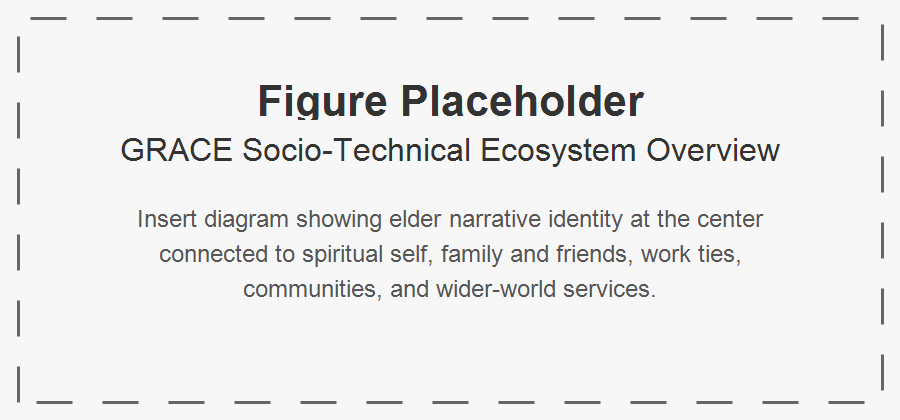
\includegraphics[keepaspectratio]{assets/figures/fig-grace-ecosystem.png}}

}

\caption{\label{fig-grace-ecosystem}Placeholder for the GRACE
socio-technical ecosystem overview.}

\end{figure}%

\subsection{A. Core Premise}\label{a.-core-premise}

GRACE is based on a simple claim: elder wellbeing emerges from the
interaction of identity, relationships, contribution, and access. A
person flourishes when they remain connected to who they are, to people
who matter, to ways of contributing, and to the broader systems that
structure everyday life.

\subsection{B. Five Relational
Domains}\label{b.-five-relational-domains}

The \textbf{spiritual-self domain} concerns inner life, faith, values,
reflection, and existential orientation. GRACE can support this domain
through reflection prompts, prayer or meditation assistance, ritual
reminders, and grief-sensitive dialogue, with the aim of sustaining
peace, hope, acceptance, and moral continuity.

The \textbf{family-and-friends domain} concerns intimate and enduring
relationships. Communication coordination, memory sharing, visit
planning, and message prompts can reinforce affection, belonging,
emotional security, and continuity of care.

The \textbf{working-colleagues domain} preserves vocational identity and
professional ties after formal employment changes or retirement.
Mentoring matches, advisory opportunities, skill sharing, and
encore-work prompts allow the elder to retain recognition, usefulness,
and role continuity.

The \textbf{community domain} includes neighborhoods, associations,
faith communities, and civic groups. Event discovery, volunteering
opportunities, group-participation support, and community connectors can
strengthen mutual aid, recognition, and collective belonging.

The \textbf{wider-world domain} connects the elder with markets,
institutions, transport, public services, and civic systems. Service
navigation, benefits assistance, transport coordination, and marketplace
access support autonomy, inclusion, and continued economic and civic
participation.

\subsection{C. Narrative Identity as System
Core}\label{c.-narrative-identity-as-system-core}

Rather than using a conventional user profile, GRACE maintains a Living
Autobiography Model. Its \textbf{temporal structure} records life
chapters, major transitions, and significant memories so current events
can be interpreted in the context of earlier vulnerabilities, strengths,
and turning points. Its \textbf{relational structure} represents
important people, social ties, and meaningful places that can guide
reconnection and place-based engagement.

The model also records \textbf{identity resources}: enduring roles,
values, beliefs, strengths, and skills. These resources help the system
align prompts with personal meaning and identify opportunities for role
continuity or contribution. Rituals and traditions provide recurring
temporal and spiritual anchors. Finally, present concerns and future
hopes keep the autobiography open rather than archival, allowing current
needs and forward-looking aims to influence support. Together, these
constructs transform biography into a living computational resource
while preserving the elder's authority over interpretation.

\subsection{D. Theater-of-Life
Perspective}\label{d.-theater-of-life-perspective}

GRACE may be understood as a theater of life: the elder is the lead
performer and author, life settings are stages, daily events are scenes,
human and AI participants form the cast, and narrative identity is the
script in progress. This metaphor is not decorative; it is a design
principle. It emphasizes authorship, visibility, and continuity.

\section{IV. The GRACE Index}\label{iv.-the-grace-index}

The GRACE Index model is summarized visually in
Fig.~\ref{fig-grace-index}, with dimensions and data sources in Table
\ref{tbl-grace-index} and scoring interpretation in Table
\ref{tbl-grace-index-zones}.

\begin{figure}

\centering{

\pandocbounded{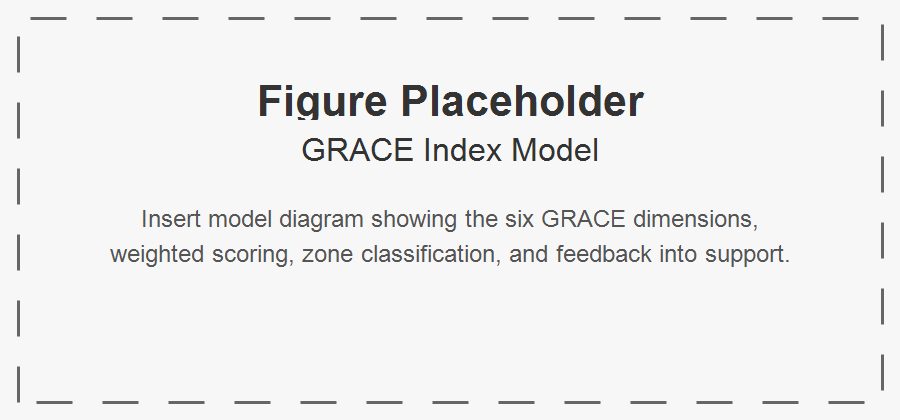
\includegraphics[keepaspectratio]{assets/figures/fig-grace-index.png}}

}

\caption{\label{fig-grace-index}Placeholder for the GRACE Index model.}

\end{figure}%

\subsection{A. Purpose}\label{a.-purpose}

The GRACE Index is a daily composite indicator designed to assess
whether a person remains ``in the zone'' of narrative selfhood. This
means the person still experiences life as meaningfully their own, even
when facing difficulty, grief, illness, or uncertainty. The index is
intended to measure narrative integrity, not merely mood or symptom
burden.

\subsection{B. Dimensions}\label{b.-dimensions}

The GRACE Index is a daily composite indicator designed to assess
whether a person remains ``in the zone'' of narrative selfhood. This
means the person still experiences life as meaningfully their own, even
when facing difficulty, grief, illness, or uncertainty. The index is
intended to measure narrative integrity, not merely mood or symptom
burden. The six dimensions, their indicators, and example data sources
are summarized in Table \ref{tbl-grace-index}.

\begin{table*}

\caption{\label{tbl-grace-index}GRACE Index dimensions, indicators, and example data sources.}

\centering{

\centering
\resizebox{\textwidth}{!}{%

\begin{tabular}{llll}
\toprule
Dimension & Description & Indicators & Example Data Sources\\
\midrule
Narrative Continuity & Sense of remaining connected to one’s life story and selfhood & felt like self, could make sense of the day, role continuity, future orientation & self-report, voice reflections, story engine outputs\\
Spiritual Grounding & Degree of inner peace, reflection, faith, or value alignment & prayer/reflection, gratitude, acceptance, values-based action & self-report, ritual logs, spiritual prompts\\
Relational Vitality & Quality of meaningful connection and belonging & meaningful contact, warmth of interaction, reciprocity, felt belonging & interaction logs, visit records, self-report\\
Contribution and Usefulness & Sense of helping, guiding, teaching, or being needed & mentoring, helping, advice-giving, feeling useful & contribution logs, task records, self-report\\
Community and World Engagement & Participation beyond the immediate self or household & event attendance, service access, neighborhood interaction, civic participation & activity logs, appointments, community records\\
\addlinespace
Adaptive Resilience & Capacity to remain centered and recover during stress & coping, help-seeking, recovery after setbacks, staying grounded & self-report, predictor features, behavior trends\\
\bottomrule
\end{tabular}
}

}

\end{table*}%

\subsection{C. Scoring Model}\label{c.-scoring-model}

Let N = Narrative Continuity; S = Spiritual Grounding; R = Relational
Vitality; C = Contribution and Usefulness; E = Community and World
Engagement; A = Adaptive Resilience.

\[G_t = 0.22N_t + 0.14S_t + 0.20R_t + 0.16C_t + 0.13E_t + 0.15A_t\]

with scores normalized to 0--100. The component weights in Table
\ref{tbl-grace-index-weights} reflect the relative importance of each
dimension to narrative selfhood.

\begin{table}

\caption{\label{tbl-grace-index-weights}Weights used to calculate the GRACE Index.}

\centering{

\centering
\resizebox{\columnwidth}{!}{%

\begin{tabular}{lr}
\toprule
Component & Weight\\
\midrule
Narrative Continuity N & 0.22\\
Spiritual Grounding S & 0.14\\
Relational Vitality R & 0.20\\
Contribution and Usefulness C & 0.16\\
Community and World Engagement E & 0.13\\
\addlinespace
Adaptive Resilience A & 0.15\\
\bottomrule
\end{tabular}
}

}

\end{table}%

\begin{table*}

\caption{\label{tbl-grace-index-zones}GRACE Index score zones and interpretations.}

\centering{

\centering
\resizebox{\textwidth}{!}{%

\begin{tabular}{lll}
\toprule
Zone & Range & Interpretation\\
\midrule
Flourishing Zone & 85–100 & strong continuity, connection, contribution, and resilience; reinforce growth and legacy opportunities\\
Stable Narrative Zone & 70–84 & stable selfhood and functioning despite ordinary challenges; maintain routines and meaningful engagement\\
Vulnerability Zone & 50–69 & early signs of drift, withdrawal, or reduced engagement; initiate gentle, targeted support\\
Disruption Zone & 30–49 & significant weakening of narrative continuity or relational vitality; escalate coordinated intervention\\
Fragmentation Risk Zone & 0–29 & severe disconnection, overwhelm, or loss of self-authorship; urgent, high-touch support with human oversight\\
\bottomrule
\end{tabular}
}

}

\end{table*}%

\subsection{D. Zone Interpretation}\label{d.-zone-interpretation}

A person may remain in a stable narrative zone even during distress if
selfhood, belonging, and meaning remain intact. As shown in Table
\ref{tbl-grace-index-zones}, the zones distinguish flourishing and
stable narrative continuity from vulnerability, disruption, and
fragmentation risk.

\section{V. Three AI-Enabled
Innovations}\label{v.-three-ai-enabled-innovations}

The three innovations form a sequence from interpretation to
anticipation and action. The Daily Story Creation Engine converts events
and reflections into a meaningful daily narrative; the Fast State
Predictor combines recent GRACE trajectories, event context, and story
features to forecast risk; and the Smart Stimulus Agent selects a
consent-aware response based on the predicted state and the elder's
preferences. The hero's-journey structure is shown in
Fig.~\ref{fig-heros-journey}, while the predictive-intervention loop is
shown in Fig.~\ref{fig-predictive-loop}.

\subsection{A. Daily Story Creation Through the Hero's
Journey}\label{a.-daily-story-creation-through-the-heros-journey}

GRACE includes a Daily Story Creation Engine that interprets everyday
life through the hero's journey. Instead of storing events as isolated
entries, it reframes them through elements such as ordinary world, call
to adventure, trial, guide, courage, insight, and return.

\begin{figure}

\centering{

\pandocbounded{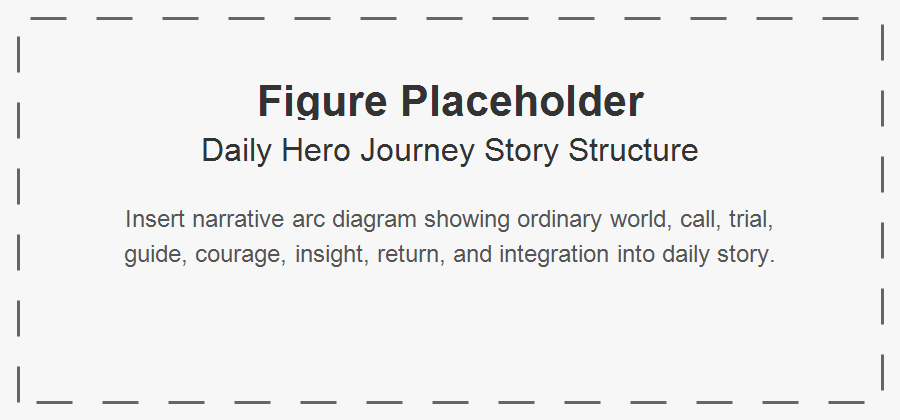
\includegraphics[keepaspectratio]{assets/figures/fig-heros-journey.png}}

}

\caption{\label{fig-heros-journey}Placeholder for the daily
hero's-journey story structure.}

\end{figure}%

\[H_t = \alpha_1T_t + \alpha_2Gd_t + \alpha_3Co_t + \alpha_4In_t\]

This mechanism is intended to buffer narrative fragmentation by
preserving meaning under adversity.

\subsection{B. AI-Based Fast State
Predictor}\label{b.-ai-based-fast-state-predictor}

GRACE includes a Fast State Predictor that forecasts near-future
wellbeing state using recent GRACE Index trajectories, event patterns,
and story features.

\begin{figure}

\centering{

\pandocbounded{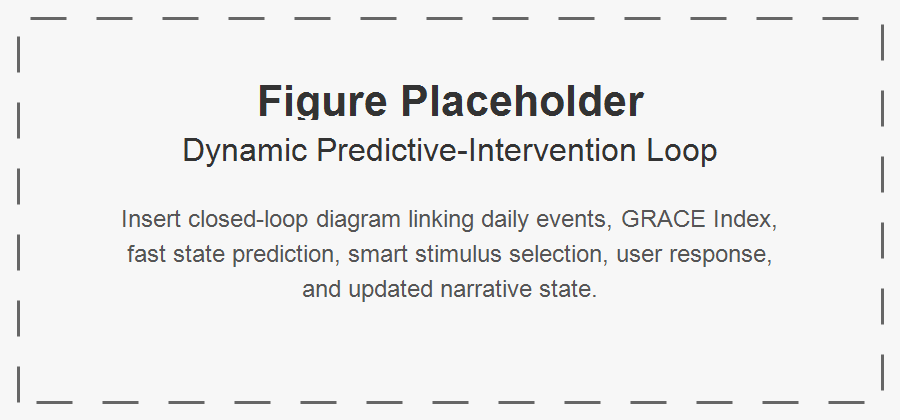
\includegraphics[keepaspectratio]{assets/figures/fig-predictive-loop.png}}

}

\caption{\label{fig-predictive-loop}Placeholder for the
predictive-intervention loop.}

\end{figure}%

\[\hat{G}_{t+\tau} = P(G_{t-\ell:t}, X_{t-\ell:t}, H_{t-\ell:t}, U_{t-\ell:t})\]

This predictor enables the system to shift from reactive monitoring to
anticipatory support.

\subsection{C. Smart Stimulus Agent}\label{c.-smart-stimulus-agent}

GRACE also includes a Smart Stimulus Agent that selects a personalized
prompt or support action based on predicted state.

\[a_t \in A = \{a^{nar}, a^{rel}, a^{spi}, a^{con}, a^{com}, a^{prac}, a^{none}\}\]

\[a_t = \pi(\hat{Z}_{t+1}, X_t, p)\]

The aim is not behavior control, but supportive intervention that helps
preserve dignity, continuity, and agency.

\section{VI. Multiagent Architecture and
Governance}\label{vi.-multiagent-architecture-and-governance}

The architecture is shown in Fig.~\ref{fig-multiagent-architecture}, and
its governance safeguards are illustrated in
Fig.~\ref{fig-governance-safeguards}.

\begin{figure}

\centering{

\pandocbounded{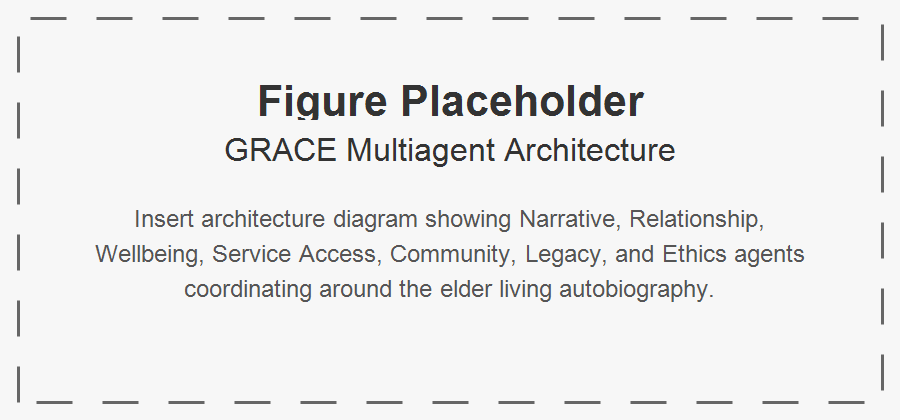
\includegraphics[keepaspectratio]{assets/figures/fig-multiagent-architecture.png}}

}

\caption{\label{fig-multiagent-architecture}Placeholder for the GRACE
multiagent architecture.}

\end{figure}%

At the core, the \textbf{Narrative Agent} maintains autobiographical
continuity, the \textbf{Wellbeing Agent} synthesizes cross-domain states
and trends, and the \textbf{Ethics and Safety Agent} applies consent
rules, constraints, approvals, and audit requirements. These agents
provide the interpretive, integrative, and governance layers of the
ecosystem.

Specialized agents connect this core to lived relationships and
services. The \textbf{Relationship Agent} monitors tie strength and
suggests reconnection; the \textbf{Spiritual Companion Agent} supports
reflection and grounding; and the \textbf{Family Coordination Agent}
assists communication, visits, and care continuity. The \textbf{Work and
Contribution Agent} identifies mentoring or service opportunities, while
the \textbf{Community Connector Agent} supports local participation. The
\textbf{Service Access Agent} assists with appointments, transport,
benefits, and institutional navigation, and the \textbf{Memory and
Legacy Agent} preserves stories and meaningful artifacts. Agent
recommendations remain subordinate to elder consent and human oversight.

\begin{figure}

\centering{

\pandocbounded{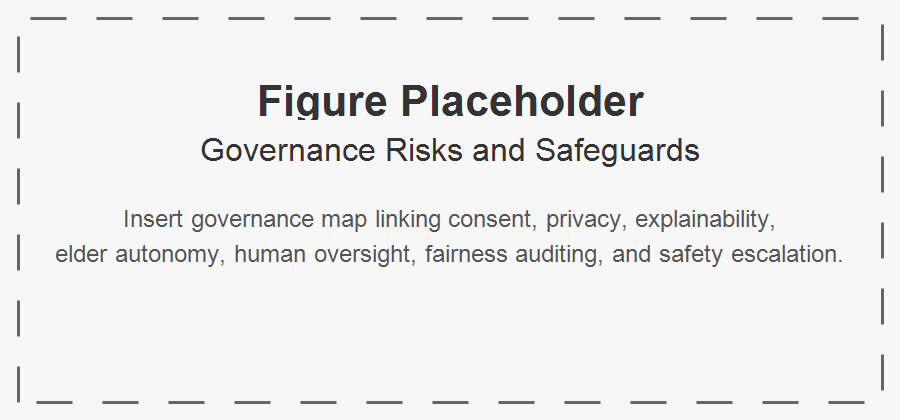
\includegraphics[keepaspectratio]{assets/figures/fig-governance-safeguards.png}}

}

\caption{\label{fig-governance-safeguards}Placeholder for governance
risks and safeguards.}

\end{figure}%

Because GRACE handles intimate autobiographical and relational data,
governance is central. \textbf{Paternalism and over-intervention} are
constrained through adjustable autonomy, rate limits, refusal, and human
override. \textbf{Narrative imposition and emotional harm} are addressed
through user-editable stories, narrative sovereignty, sensitivity rules,
and careful timing. \textbf{Privacy breaches and family misuse} require
encryption, granular permissions, consent-based sharing, and elder-first
governance. \textbf{Opaque or biased prediction} requires explanation,
subgroup validation, and fairness audits. Finally, connection-first
policies should prevent dependency on AI mediation and preserve direct
human relationships.

\section{VII. Agent-Based Simulation
Design}\label{vii.-agent-based-simulation-design}

The simulation structure is shown in
Fig.~\ref{fig-simulation-structure}, with conditions in Table
\ref{tbl-simulation-conditions}, hypotheses in Table
\ref{tbl-simulation-hypotheses}, variables in Table
\ref{tbl-simulation-variables}, and outcome metrics in Table
\ref{tbl-simulation-outcomes}.

\subsection{A. Objective}\label{a.-objective}

Before real-world deployment, the three innovations should be evaluated
in simulation.

\begin{figure}

\centering{

\pandocbounded{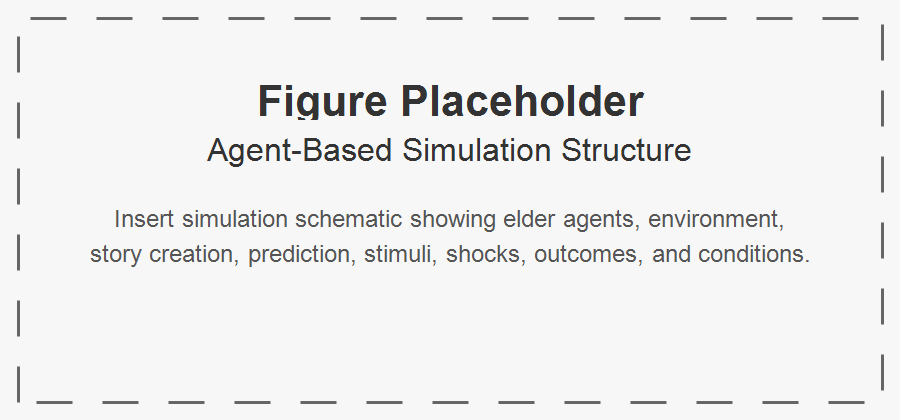
\includegraphics[keepaspectratio]{assets/figures/fig-simulation-structure.png}}

}

\caption{\label{fig-simulation-structure}Placeholder for the agent-based
simulation structure.}

\end{figure}%

\subsection{B. Agents}\label{b.-agents}

Elder Agent; Narrative Agent; Predictor Agent; Stimulus Agent; Social
Tie Agents; Environment Agent.

\subsection{C. State Representation}\label{c.-state-representation}

\[X_{i,t} = [N_{i,t}, S_{i,t}, R_{i,t}, C_{i,t}, E_{i,t}, A_{i,t}]\]

\[G_{i,t} = 0.22N_{i,t} + 0.14S_{i,t} + 0.20R_{i,t} + 0.16C_{i,t} + 0.13E_{i,t} + 0.15A_{i,t}\]

\[X_{i,t+1} = f(X_{i,t}, U_{i,t}, H_{i,t}, A_{i,t}^{stim}, \varepsilon_{i,t})\]

\begin{table*}

\caption{\label{tbl-simulation-conditions}Simulation conditions for evaluating GRACE innovations.}

\centering{

\centering
\resizebox{\textwidth}{!}{%

\begin{tabular}{lllll}
\toprule
Condition & Story & Prediction & Stimulus & Expectation\\
\midrule
Baseline & No & No & No & monitoring only\\
Story Only & Yes & No & No & improved narrative continuity\\
Story + Prediction & Yes & Yes & No & improved early risk detection\\
Full GRACE & Yes & Yes & Yes & highest stability and fastest recovery\\
\bottomrule
\end{tabular}
}

}

\end{table*}%

\begin{table*}

\caption{\label{tbl-simulation-hypotheses}Simulation hypotheses for GRACE.}

\centering{

\centering
\resizebox{\textwidth}{!}{%

\begin{tabular}{ll}
\toprule
Hypothesis & Expectation\\
\midrule
H1 & Story creation increases Narrative Continuity relative to baseline\\
H2 & Fast prediction improves early detection of decline\\
H3 & Smart stimuli reduce time spent in low GRACE zones\\
H4 & Full GRACE yields highest average GRACE Index\\
H5 & Full GRACE reduces recovery time after adverse shocks\\
\bottomrule
\end{tabular}
}

}

\end{table*}%

\begin{table*}

\caption{\label{tbl-simulation-variables}State and derived variables tracked in the simulation.}

\centering{

\centering
\resizebox{\textwidth}{!}{%

\begin{tabular}{llll}
\toprule
Variable & Name & Type & Function\\
\midrule
N & Narrative Continuity & state variable & tracks self-story coherence\\
S & Spiritual Grounding & state variable & tracks inner steadiness\\
R & Relational Vitality & state variable & tracks connection quality\\
C & Contribution and Usefulness & state variable & tracks perceived usefulness\\
E & Community and World Engagement & state variable & tracks external participation\\
\addlinespace
A & Adaptive Resilience & state variable & tracks coping and recovery\\
G & GRACE Index & composite metric & primary wellbeing outcome\\
H & Heroic Integration Score & derived metric & measures successful narrative reframing\\
\bottomrule
\end{tabular}
}

}

\end{table*}%

\begin{table*}

\caption{\label{tbl-simulation-outcomes}Outcome metrics used to evaluate the simulation.}

\centering{

\centering
\resizebox{\textwidth}{!}{%

\begin{tabular}{lll}
\toprule
Variable & Type & Function\\
\midrule
Stable-Zone Days & outcome metric & proportion of days with G >= 70; assesses sustained wellbeing\\
Vulnerable/Disrupted Days & outcome metric & proportion of days with G < 70; assesses instability\\
Recovery Time & outcome metric & days to return to stable zone after shock; assesses resilience\\
Reframing Success & outcome metric & proportion of adverse days with high H; assesses story engine effect\\
Intervention Efficiency & outcome metric & gain in G per stimulus action; assesses stimulus value\\
\bottomrule
\end{tabular}
}

}

\end{table*}%

\section{VIII. Technology and Society
Implications}\label{viii.-technology-and-society-implications}

\subsection{A. From Monitoring to
Meaning}\label{a.-from-monitoring-to-meaning}

Many existing systems for older adults are designed around surveillance,
compliance, and risk reduction. Although these functions are often
necessary, they can narrow the social meaning of technology to
observation and behavioral management. GRACE suggests a different
orientation: intelligent systems should also support meaning-making,
narrative continuity, and relationship quality. This matters because
technologies do not merely assist users; they also shape how users are
socially perceived. A system that frames older adults mainly as
vulnerable subjects of monitoring may reinforce dependency narratives.
By contrast, a system that recognizes them as authors, contributors, and
relational beings may support dignity and public visibility.

\subsection{B. The Social Construction of Aging Through
Technology}\label{b.-the-social-construction-of-aging-through-technology}

Technologies embody assumptions about the populations they serve. In
aging contexts, these assumptions often center decline, burden, and
incapacity. Such framings can indirectly reproduce ageism by embedding
deficit-oriented views of later life into interfaces, workflows, and
service logics. GRACE instead frames later life as a stage of ongoing
identity development, contribution, and relational growth. This shift
has implications beyond design. It suggests that socio-technical systems
should not merely adapt to older adults as they are socially classified,
but should also challenge reductive classifications that limit
participation and agency.

\subsection{C. Narrative Data as a New Category of Sensitive
Data}\label{c.-narrative-data-as-a-new-category-of-sensitive-data}

GRACE relies on autobiographical, relational, and interpretive data in
addition to behavioral and service data. This class of information is
especially sensitive because it concerns identity, memory, grief,
values, and social bonds. Conventional privacy models may be
insufficient for such data because the issue is not only exposure, but
interpretation and authorship. Questions arise regarding who owns a life
story representation, who may correct or extend it, and how conflicting
interpretations should be handled when family members or institutions
are involved. The use of narrative data therefore requires governance
structures that protect not only privacy, but also identity integrity.

\subsection{D. Prediction, Intervention, and the Risk of
Paternalism}\label{d.-prediction-intervention-and-the-risk-of-paternalism}

The Fast State Predictor and Smart Stimulus Agent introduce anticipatory
action into elder-oriented systems. While this can improve support, it
also creates the risk of paternalism. Predictions may be used to steer
behavior in ways that are insufficiently transparent or insufficiently
aligned with the elder's own intentions. In contexts where older adults
are already socially positioned as dependent, such interventions may
amplify rather than reduce power asymmetries. GRACE therefore implies
that predictive systems should be explainable, consent-aware, adjustable
in intensity, and always open to refusal or override. The goal is not to
optimize the person, but to support the person's own authorship.

\subsection{E. Human-Centered AI in Socially Embedded
Contexts}\label{e.-human-centered-ai-in-socially-embedded-contexts}

GRACE contributes to human-centered AI by expanding what counts as
success in intelligent systems. Reliability, safety, and performance
remain necessary, but they are not sufficient in socially embedded
domains such as aging. Systems should also be evaluated according to
whether they preserve agency, dignity, self-interpretation, reciprocity,
and belonging. In this sense, GRACE argues for a broader evaluative
framework for AI in society: one that includes effects on identity and
relational life alongside traditional technical metrics.

\subsection{F. Social Infrastructure and
Inclusion}\label{f.-social-infrastructure-and-inclusion}

Older adult wellbeing depends not only on internal state or family
support, but also on access to social infrastructure, including
transportation, public services, community groups, and marketplaces.
GRACE highlights that intelligent support systems should therefore
function not merely as private assistants, but as bridges to
institutional and civic participation. This has policy implications.
Public-interest technologies for aging should be designed to support
inclusion, not just care; participation, not just monitoring; and
contribution, not just dependency management.

\subsection{G. Implications for Technology
Governance}\label{g.-implications-for-technology-governance}

From a technology-and-society perspective, GRACE suggests five
governance principles for elder-oriented AI. First, narrative
sovereignty: the elder retains primary authority over their life story
representation. Second, consentful prediction: predictive analytics must
be understandable, optional, and bounded in use. Third, non-manipulative
intervention: prompts and actions should support rather than coerce.
Fourth, relational accountability: system actions should be evaluated
for their effects on family, community, and institutional relationships.
Fifth, dignity-centered evaluation: success should include preservation
of selfhood, not only efficiency or compliance.

\subsection{H. Broader Relevance}\label{h.-broader-relevance}

Although GRACE is developed for older adults, its implications extend to
other domains in which wellbeing depends on identity continuity and
social participation, including disability support, chronic illness,
rehabilitation, and mental health recovery. More broadly, the framework
suggests that intelligent socio-technical systems should be designed not
only to predict and intervene, but also to help persons remain present
in their own lives.

\section{IX. Discussion}\label{ix.-discussion}

Taken together, Fig.~\ref{fig-grace-ecosystem},
Fig.~\ref{fig-multiagent-architecture}, Fig.~\ref{fig-predictive-loop},
Fig.~\ref{fig-heros-journey}, Fig.~\ref{fig-grace-index},
Fig.~\ref{fig-simulation-structure},
Fig.~\ref{fig-governance-safeguards}, and the quantitative tables show
that GRACE is not merely a collection of tools, but an integrated
socio-technical ecosystem.

GRACE reframes elder-oriented AI away from narrow models of surveillance
and deficit management. Its central contribution is to treat older
adults as ongoing authors of life rather than passive subjects of care.
This reframing changes the role of intelligent systems. Instead of
merely detecting problems or enforcing routines, such systems can
support meaning, relationship quality, contribution, and continuity of
self.

The GRACE Index is important in this regard because it shifts
measurement away from symptom burden alone and toward narrative
integrity. A person may be grieving, ill, or facing uncertainty while
still remaining deeply connected to selfhood, belonging, and purpose.
Conventional metrics may not capture this distinction. By contrast, the
GRACE Index is intended to identify whether the person remains ``in the
zone'' of narrative selfhood, thereby enabling support that is more
humane and context-sensitive.

The three added innovations extend this contribution. The Daily Story
Creation Engine offers a computational mechanism for narrative
reframing. The Fast State Predictor moves the system from reactive to
anticipatory operation. The Smart Stimulus Agent transforms prediction
into practical support. In combination, these mechanisms suggest a new
class of elder-oriented intelligent systems: systems that are
reflective, predictive, and supportive, while remaining grounded in
dignity and agency.

For IEEE audiences, the broader implication is that intelligent systems
in socially sensitive settings should be evaluated not only by technical
performance, but also by their effects on identity, autonomy, and social
life. GRACE therefore contributes to ongoing conversations about
human-centered AI, algorithmic governance, and the social
responsibilities of digital infrastructure.

The proposed agent-based simulation design provides a useful
intermediate step before real-world deployment. It allows key questions
to be examined under controlled conditions: whether narrative reframing
buffers decline, whether predictive models can identify vulnerability
early, and whether stimulus policies improve recovery without becoming
intrusive. It also enables examination of governance concerns such as
intervention thresholds, uncertainty handling, and the trade-off between
support and paternalism.

At the same time, GRACE should be understood as a framework rather than
a finished system. Its value lies in offering a coherent socio-technical
direction for future work at the intersection of aging, AI, and
community computing.

\section{X. Limitations and Future
Work}\label{x.-limitations-and-future-work}

This paper is conceptual and simulation-oriented. Several limitations
should therefore be acknowledged.

First, the GRACE Index is proposed as a theoretically grounded composite
measure, but its weighting scheme and dimensional structure have not yet
been empirically validated. The model should be treated as provisional
until psychometric testing, longitudinal analysis, and user-centered
validation are conducted.

Second, the Daily Story Creation Engine, Fast State Predictor, and Smart
Stimulus Agent are presented as design innovations, not as fully
implemented and tested modules. Their actual effectiveness will depend
on interface quality, data quality, personalization logic, and the
degree to which users perceive them as supportive rather than intrusive.

Third, the proposed simulation is an abstraction of real life. Although
simulation can help evaluate mechanisms and explore policy behavior, it
cannot fully represent the emotional, cultural, and relational
complexity of lived aging. Real-world evaluation with older adults,
families, and community organizations remains essential.

Fourth, the framework may require substantial cultural adaptation.
Narrative identity, spirituality, family expectations, contribution
norms, and attitudes toward AI vary across settings. A system designed
around autobiographical continuity and relational support must therefore
be locally interpretable and culturally responsive.

Fifth, governance challenges remain significant. The use of
autobiographical and predictive data introduces risks related to
privacy, bias, paternalism, narrative imposition, and over-intervention.
Future work should address these issues through fairness testing,
explainability design, participatory governance, and careful consent
models.

Future research should proceed along at least six directions: 1.
participatory co-design with older adults, caregivers, and community
stakeholders; 2. prototype implementation of the GRACE ecosystem and
GRACE Index interfaces; 3. simulation execution and reporting to
evaluate the three innovations under controlled scenarios; 4.
psychometric validation of the GRACE Index across diverse elder
populations; 5. pilot deployment studies to assess usability,
acceptability, and perceived dignity impact; and 6. governance and
fairness analysis focused on predictive intervention, consent, and
relational accountability.

These steps are necessary to move GRACE from a conceptual
socio-technical framework toward a validated and ethically robust
intelligent ecosystem.

\section{XI. Conclusion}\label{xi.-conclusion}

GRACE proposes a narrative-centered socio-technical ecosystem for elder
wellbeing. By integrating relationship quality, autobiographical
continuity, predictive modeling, and anticipatory intervention, it
offers an alternative to deficit-oriented aging technologies. Rather
than viewing older adults primarily through decline, risk, and service
dependency, GRACE understands them as persons who continue to live,
interpret, and contribute within unfolding life stories.

The framework contributes four main ideas: a relational and narrative
model of elder wellbeing; the GRACE Index as a daily measure of
narrative selfhood; three AI-enabled mechanisms for story creation,
prediction, and supportive intervention; and an agent-based simulation
design for structured evaluation. Together, these elements suggest that
intelligent systems for older adults should be designed not only to
manage risk, but also to sustain dignity, reciprocity, participation,
and the ongoing authorship of life.

More broadly, GRACE argues that the future of elder-oriented AI should
be socio-technical rather than merely technical, and human-centered in a
deep sense: not simply usable, but respectful of identity, meaning, and
relationship. If developed responsibly, systems like GRACE may help
ensure that digital innovation in aging supports not only longer life,
but more connected, authored, and enriched life.

\section*{References}\label{references}
\addcontentsline{toc}{section}{References}

\protect\phantomsection\label{refs}
\begin{CSLReferences}{0}{0}
\bibitem[\citeproctext]{ref-un2024wpp}
\CSLLeftMargin{{[}1{]} }%
\CSLRightInline{United Nations Department of Economic and Social
Affairs, Population Division, {``World population prospects 2024:
Summary of results,''} United Nations, New York, 2024 {[}Online{]}.
Available:
\url{https://population.un.org/wpp/assets/Files/WPP2024_Summary-of-Results.pdf}}

\bibitem[\citeproctext]{ref-baig2019wearable}
\CSLLeftMargin{{[}2{]} }%
\CSLRightInline{M. M. Baig, S. Afifi, H. GholamHosseini, and F. Mirza,
{``\href{https://doi.org/10.1007/s10916-019-1365-7}{A systematic review
of wearable sensors and {IoT}-based monitoring applications for older
adults: A focus on ageing population and independent living},''}
\emph{Journal of Medical Systems}, vol. 43, no. 8, p. 233, 2019. }

\bibitem[\citeproctext]{ref-vines2015age}
\CSLLeftMargin{{[}3{]} }%
\CSLRightInline{J. Vines, G. Pritchard, P. Wright, P. Olivier, and K.
Brittain, {``\href{https://doi.org/10.1145/2696867}{An age-old problem:
Examining the discourses of ageing in {HCI} and strategies for future
research},''} \emph{ACM Transactions on Computer-Human Interaction},
vol. 22, no. 1, pp. 2:1--2:27, 2015. }

\bibitem[\citeproctext]{ref-holt2010social}
\CSLLeftMargin{{[}4{]} }%
\CSLRightInline{J. Holt-Lunstad, T. B. Smith, and J. B. Layton,
{``\href{https://doi.org/10.1371/journal.pmed.1000316}{Social
relationships and mortality risk: A meta-analytic review},''} \emph{PLOS
Medicine}, vol. 7, no. 7, p. e1000316, 2010. }

\bibitem[\citeproctext]{ref-mcadams1992generativity}
\CSLLeftMargin{{[}5{]} }%
\CSLRightInline{D. P. McAdams and E. de St. Aubin,
{``\href{https://doi.org/10.1037/0022-3514.62.6.1003}{A theory of
generativity and its assessment through self-report, behavioral acts,
and narrative themes in autobiography},''} \emph{Journal of Personality
and Social Psychology}, vol. 62, no. 6, pp. 1003--1015, 1992. }

\bibitem[\citeproctext]{ref-mcadams2013narrative}
\CSLLeftMargin{{[}6{]} }%
\CSLRightInline{D. P. McAdams and K. C. McLean,
{``\href{https://doi.org/10.1177/0963721413475622}{Narrative
identity},''} \emph{Current Directions in Psychological Science}, vol.
22, no. 3, pp. 233--238, 2013. }

\bibitem[\citeproctext]{ref-sixsmith2013technologies}
\CSLLeftMargin{{[}7{]} }%
\CSLRightInline{A. Sixsmith and G. Gutman, Eds., \emph{Technologies for
active aging}. New York: Springer, 2013. }

\bibitem[\citeproctext]{ref-czaja2006factors}
\CSLLeftMargin{{[}8{]} }%
\CSLRightInline{S. J. Czaja \emph{et al.},
{``\href{https://doi.org/10.1037/0882-7974.21.2.333}{Factors predicting
the use of technology: Findings from the center for research and
education on aging and technology enhancement},''} \emph{Psychology and
Aging}, vol. 21, no. 2, pp. 333--352, 2006. }

\bibitem[\citeproctext]{ref-mitzner2010older}
\CSLLeftMargin{{[}9{]} }%
\CSLRightInline{T. L. Mitzner \emph{et al.},
{``\href{https://doi.org/10.1016/j.chb.2010.06.020}{Older adults talk
technology: Technology usage and attitudes},''} \emph{Computers in Human
Behavior}, vol. 26, no. 6, pp. 1710--1721, 2010. }

\bibitem[\citeproctext]{ref-cacioppo2009isolation}
\CSLLeftMargin{{[}10{]} }%
\CSLRightInline{J. T. Cacioppo and L. C. Hawkley,
{``\href{https://doi.org/10.1016/j.tics.2009.06.005}{Perceived social
isolation and cognition},''} \emph{Trends in Cognitive Sciences}, vol.
13, no. 10, pp. 447--454, 2009. }

\bibitem[\citeproctext]{ref-cornwell2009disconnectedness}
\CSLLeftMargin{{[}11{]} }%
\CSLRightInline{E. Y. Cornwell and L. J. Waite,
{``\href{https://doi.org/10.1177/002214650905000103}{Social
disconnectedness, perceived isolation, and health among older
adults},''} \emph{Journal of Health and Social Behavior}, vol. 50, no.
1, pp. 31--48, 2009. }

\bibitem[\citeproctext]{ref-berkman2000integration}
\CSLLeftMargin{{[}12{]} }%
\CSLRightInline{L. F. Berkman, T. Glass, I. Brissette, and T. E. Seeman,
{``\href{https://doi.org/10.1016/S0277-9536(00)00065-4}{From social
integration to health: Durkheim in the new millennium},''} \emph{Social
Science \& Medicine}, vol. 51, no. 6, pp. 843--857, 2000. }

\bibitem[\citeproctext]{ref-mcadams2001psychology}
\CSLLeftMargin{{[}13{]} }%
\CSLRightInline{D. P. McAdams,
{``\href{https://doi.org/10.1037/1089-2680.5.2.100}{The psychology of
life stories},''} \emph{Review of General Psychology}, vol. 5, no. 2,
pp. 100--122, 2001. }

\bibitem[\citeproctext]{ref-habermas2000life}
\CSLLeftMargin{{[}14{]} }%
\CSLRightInline{T. Habermas and S. Bluck,
{``\href{https://doi.org/10.1037/0033-2909.126.5.748}{Getting a life:
The emergence of the life story in adolescence},''} \emph{Psychological
Bulletin}, vol. 126, no. 5, pp. 748--769, 2000. }

\bibitem[\citeproctext]{ref-singer2004identity}
\CSLLeftMargin{{[}15{]} }%
\CSLRightInline{J. A. Singer,
{``\href{https://doi.org/10.1111/j.0022-3506.2004.00268.x}{Narrative
identity and meaning making across the adult lifespan: An
introduction},''} \emph{Journal of Personality}, vol. 72, no. 3, pp.
437--460, 2004. }

\bibitem[\citeproctext]{ref-langi2025author}
\CSLLeftMargin{{[}16{]} }%
\CSLRightInline{A. Z. R. Langi, \emph{The author of yourself: A
practical guide to writing the story of your life}. 2025. }

\bibitem[\citeproctext]{ref-butler1963review}
\CSLLeftMargin{{[}17{]} }%
\CSLRightInline{R. N. Butler,
{``\href{https://doi.org/10.1080/00332747.1963.11023339}{The life
review: An interpretation of reminiscence in the aged},''}
\emph{Psychiatry}, vol. 26, no. 1, pp. 65--76, 1963. }

\bibitem[\citeproctext]{ref-bohlmeijer2007reminiscence}
\CSLLeftMargin{{[}18{]} }%
\CSLRightInline{E. Bohlmeijer, M. Roemer, P. Cuijpers, and F. Smit,
{``\href{https://doi.org/10.1080/13607860600963547}{The effects of
reminiscence on psychological well-being in older adults: A
meta-analysis},''} \emph{Aging \& Mental Health}, vol. 11, no. 3, pp.
291--300, 2007. }

\bibitem[\citeproctext]{ref-erikson1982cycle}
\CSLLeftMargin{{[}19{]} }%
\CSLRightInline{E. H. Erikson, \emph{The life cycle completed}. New
York: W. W. Norton, 1982. }

\bibitem[\citeproctext]{ref-morrowhowell2017engagement}
\CSLLeftMargin{{[}20{]} }%
\CSLRightInline{N. Morrow-Howell, E. Gonzales, R. Harootyan, Y. Lee, and
B. Lindberg,
{``\href{https://doi.org/10.1080/01634372.2016.1275912}{Approaches,
policies, and practices to support the productive engagement of older
adults},''} \emph{Journal of Gerontological Social Work}, vol. 60, no.
3, pp. 193--200, 2017. }

\bibitem[\citeproctext]{ref-gurstein2007community}
\CSLLeftMargin{{[}21{]} }%
\CSLRightInline{M. Gurstein, \emph{What is community informatics (and
why does it matter)?} Milan: Polimetrica, 2007. }

\bibitem[\citeproctext]{ref-jennings1998roadmap}
\CSLLeftMargin{{[}22{]} }%
\CSLRightInline{N. R. Jennings, K. Sycara, and M. Wooldridge,
{``\href{https://doi.org/10.1023/A:1010090405266}{A roadmap of agent
research and development},''} \emph{Autonomous Agents and Multi-Agent
Systems}, vol. 1, no. 1, pp. 7--38, 1998. }

\bibitem[\citeproctext]{ref-wooldridge2009introduction}
\CSLLeftMargin{{[}23{]} }%
\CSLRightInline{M. Wooldridge, \emph{An introduction to MultiAgent
systems}, 2nd ed. Chichester: Wiley, 2009. }

\bibitem[\citeproctext]{ref-shneiderman2020human}
\CSLLeftMargin{{[}24{]} }%
\CSLRightInline{B. Shneiderman,
{``\href{https://doi.org/10.1080/10447318.2020.1741118}{Human-centered
artificial intelligence: Reliable, safe \& trustworthy},''}
\emph{International Journal of Human--Computer Interaction}, vol. 36,
no. 6, pp. 495--504, 2020. }

\end{CSLReferences}


% Can use something like this to put references on a page
% by themselves when using endfloat and the captionsoff option.
\ifCLASSOPTIONcaptionsoff
  \newpage
\fi

% trigger a \newpage just before the given reference
% number - used to balance the columns on the last page
% adjust value as needed - may need to be readjusted if
% the document is modified later
%\IEEEtriggeratref{8}
% The "triggered" command can be changed if desired:
%\IEEEtriggercmd{\enlargethispage{-5in}}

% Uncomment when use biblatex with style=ieee
%\renewcommand{\bibfont}{\footnotesize} % for IEEE bibfont size

\pagebreak[3]
\begin{IEEEbiography}[
\includegraphics{azrl.png}]{David Folio}
Use \texttt{IEEEbiography} with figure as option and the author name as
the argument followed by the biography text.
\end{IEEEbiography}
\begin{IEEEbiographynophoto}{John Doe}
Use \texttt{IEEEbiographynophoto} and the author name as the argument
followed by the biography text.
\end{IEEEbiographynophoto}
% that's all folks
\end{document}

